\begin{surferPage}{Quíntica con 15 picos}
  Esta superficie de grado $5$ (quíntica) tiene $15$ singularidades del tipo picos.
  Ésta, junto con una serie de superficies, fue dada por Oliver Labs en uno de sus artículos en 2005.
  Es claro que cinco de los picos difieren de los otros diez. Esta diferencia se
  puede notar a su vez, si hiciéramos un análisis de función a la ecuación. Así es como hoy
  en día existe una subclasificación de las singularidades de tipo pico.
  
       \vspace*{-0.3em}
    \begin{center}
      \begin{tabular}{c@{\qquad}c}
        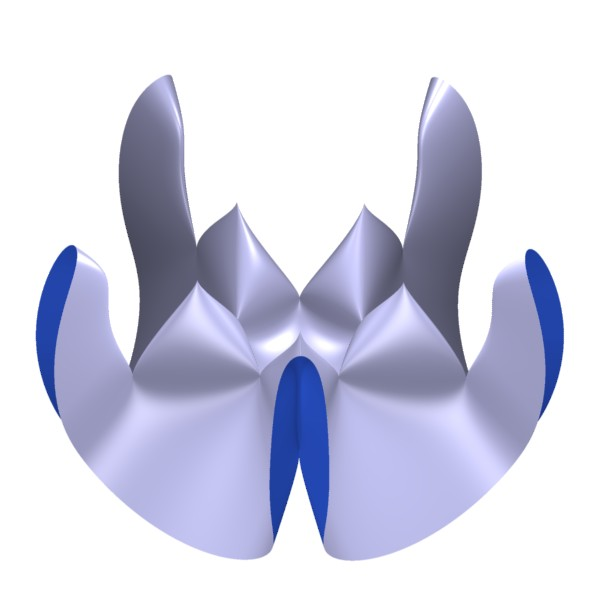
\includegraphics[height=1.2cm]{../../common/images/dessins_quint_15a2}
        &
        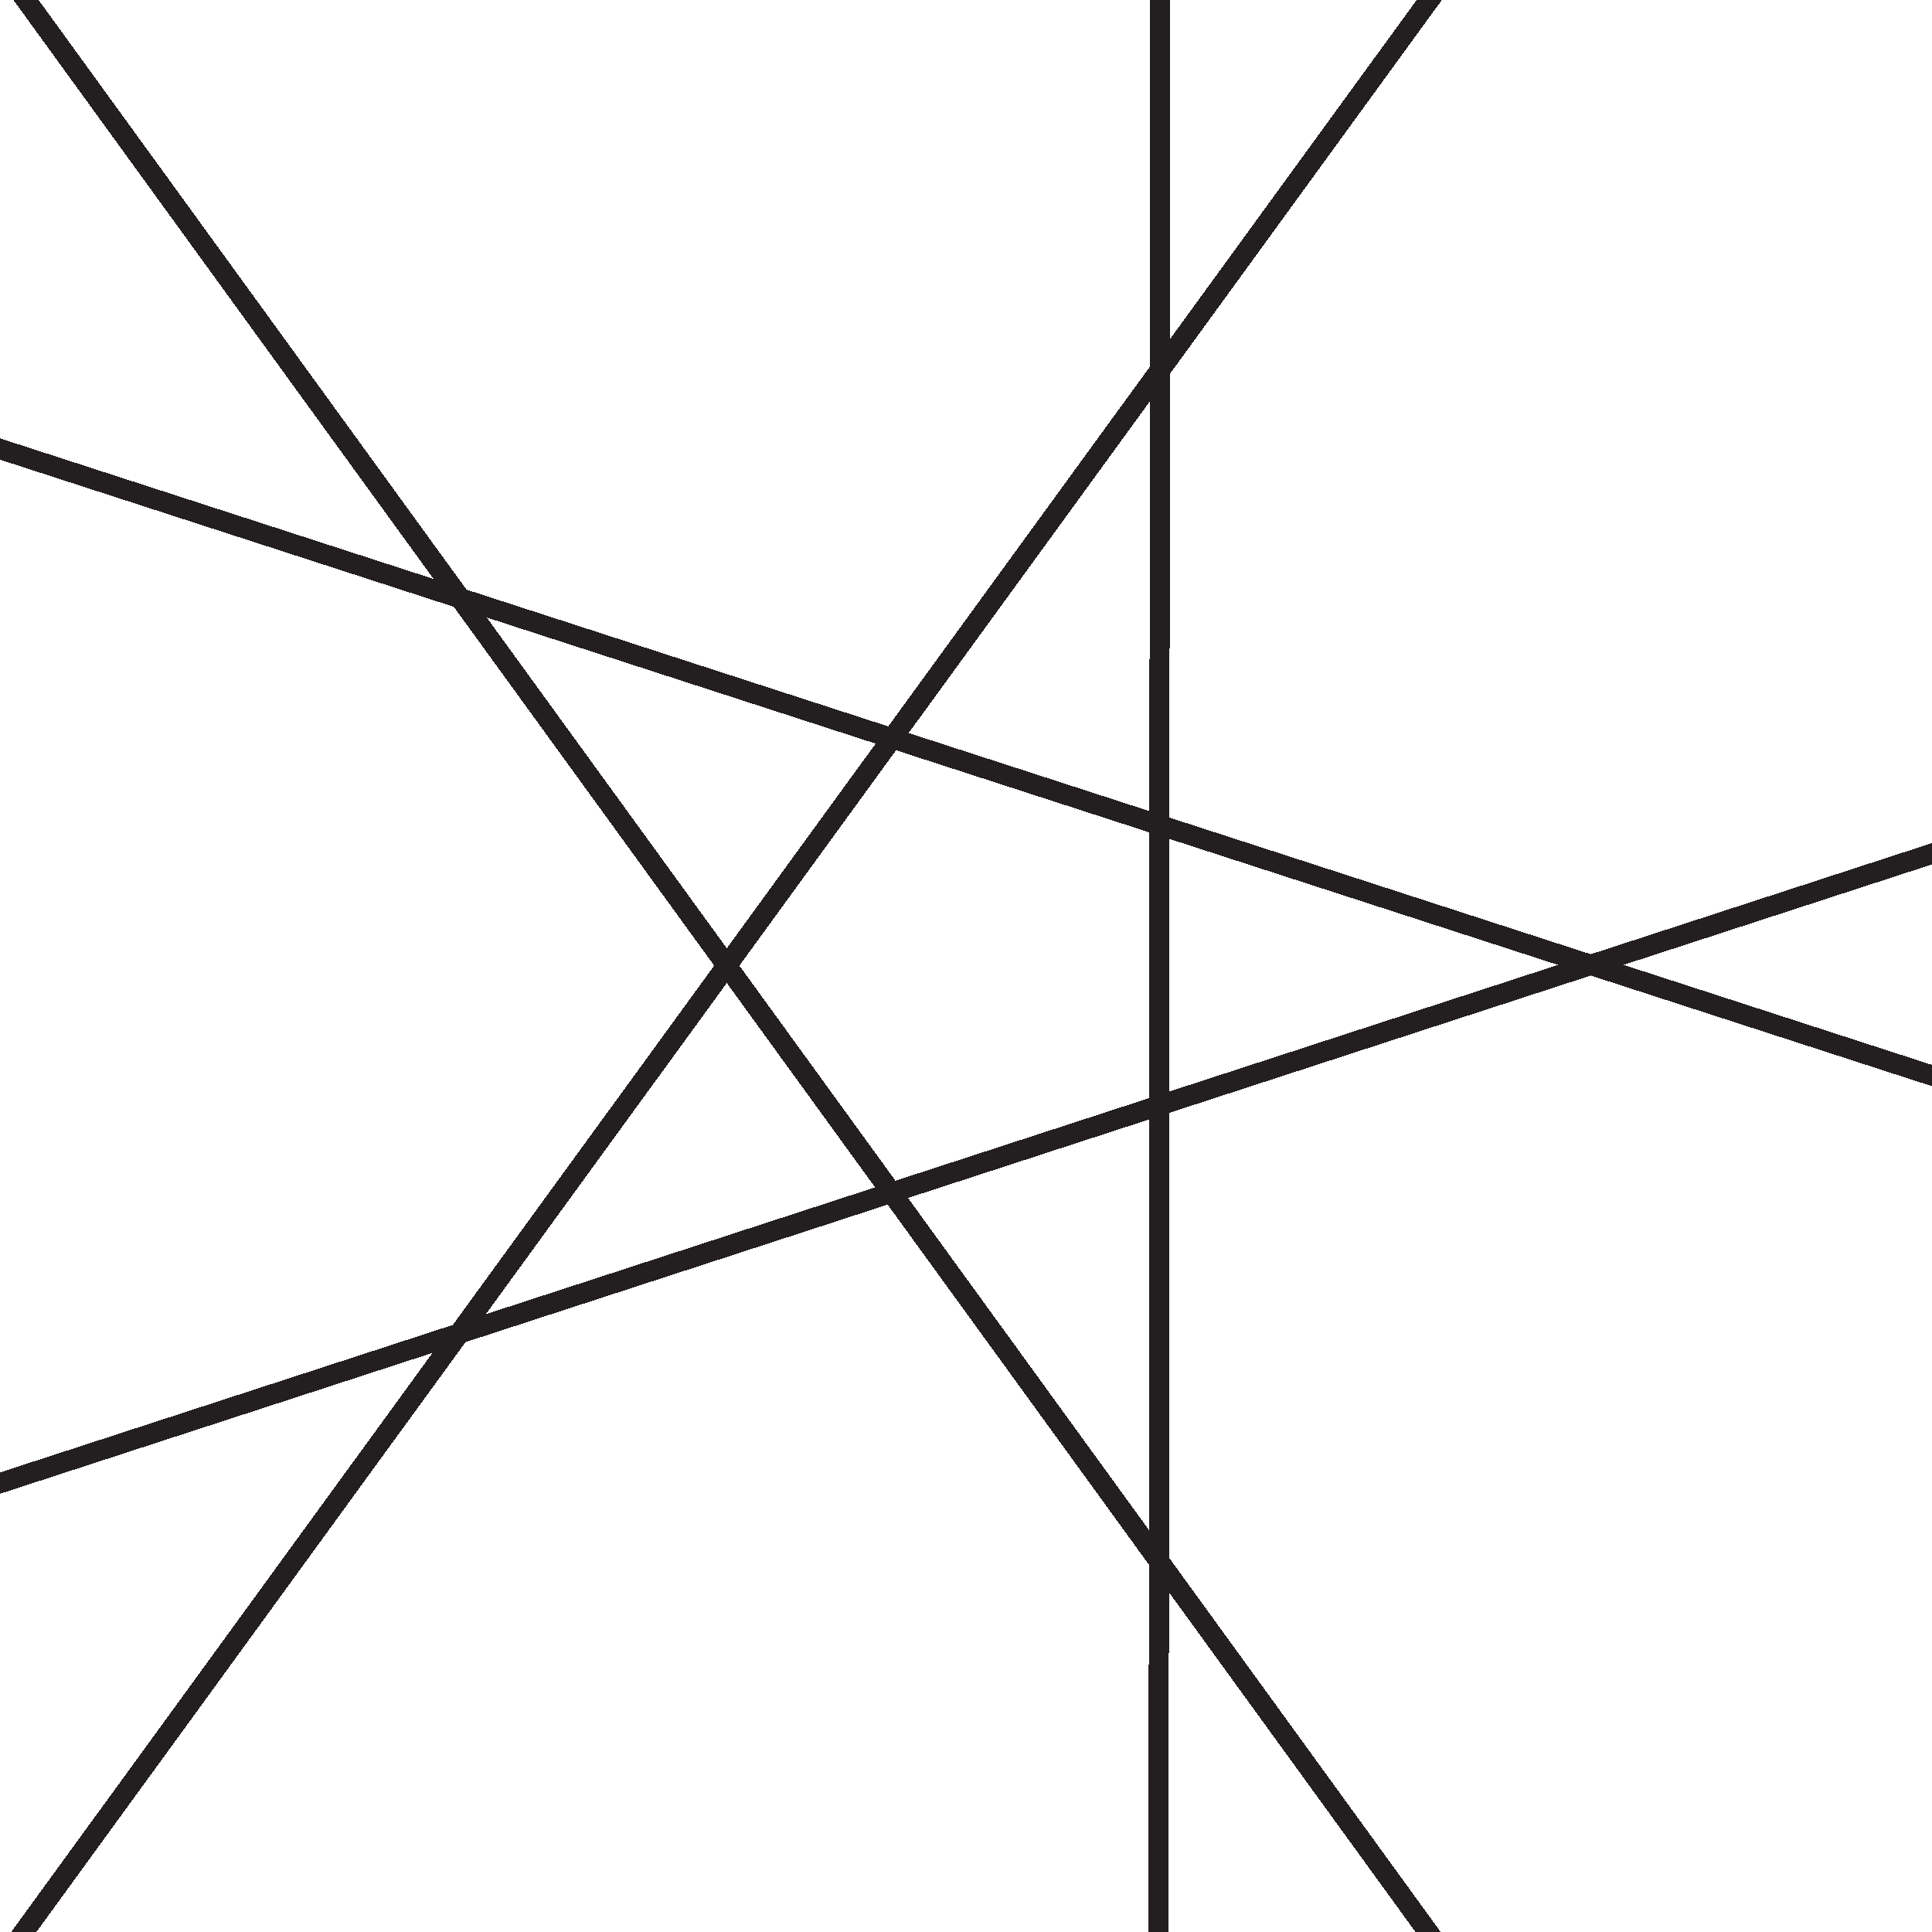
\includegraphics[height=1.2cm]{../../common/images/rp5.pdf}
      \end{tabular}
    \end{center}
    \vspace*{-0.3em}    
    
    Esta superficie tiene una ecuación de la forma
    $S_5(x,y) + t(z)=0$, donde $S_5(x,y)$ es un pentágono regular
    (imagen de la derecha) y $t(z)$ es una variante de los polinomios
    de Tchebychev, que ya hemos mencionado varias veces.
    
    Otra quíntica con $15$ picos (la de la izquierda) fue construida
    por Wolf Barth; está relacionada con la cúbica de Clebsch
    (la de la derecha), como se puede observar en la imagen del medio:

    \vspace*{-0.3em}
    \begin{center}
      \begin{tabular}{c@{\quad}c@{\quad}c}
        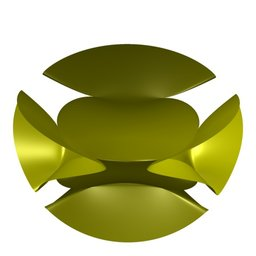
\includegraphics[height=1.2cm]{../../common/images/barthquintic_green}
        &
        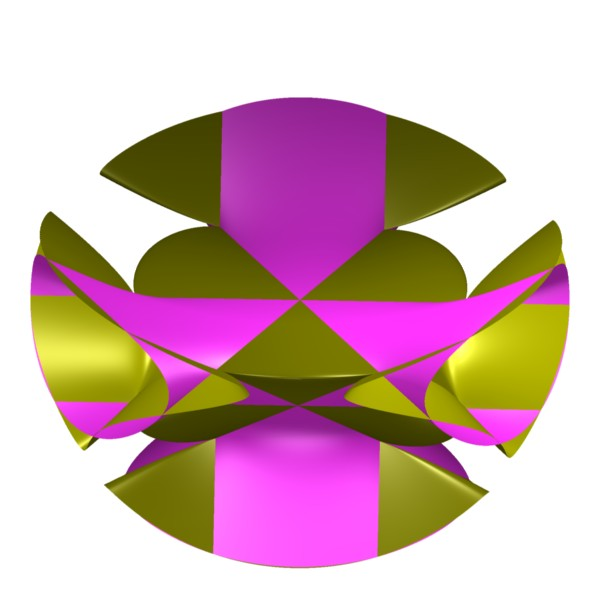
\includegraphics[height=1.2cm]{../../common/images/barthquintic_clebschcubic}
        &
        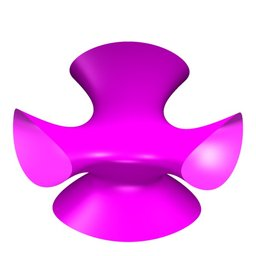
\includegraphics[height=1.2cm]{../../common/images/clebschcubic_pink}
      \end{tabular}
    \end{center}
    \vspace*{-0.3em}
\end{surferPage}
